\section{Description}
		
		zkInterface is a purely functional interface for zero-knowledge systems that enables cross-language interoperability via dynamic linking and shared memory. The current version, even if limiting, creates an interface based on R1CS formatting and offers the ability to abstractly craft a constraint system building from different components, possibly written in different frameworks, by determining how data should be written and read. 
		
		It can also be seen as a design tool for improved generation of constraints and usability, analogous to a portable binary format, since one can parametrize the functions calls and easily compose different functions, or components, that are not directly compatible.
		
		It is important to point out that the interface can be called both to write a request or read a response by having an encoder at the front-end  and a decoder at the back-end. 
		
		\paragraph{Main functionality.}
		
		The interface works across every zero-knowledge front-end and back-end, minimizing, when possible, the overhead of using a general format. This is achieved in several ways:
        
        \begin{itemize}
			\item By using a protoboard-like method for shared memory allocation, and thus preventing double-copying the data unnecessarily.
			\item By parametrizing the function calls to the different components so to take advantage of the specific context underlying those components.
			\item By using FlatBuffers, an efficient cross platform serialization library for different languages. This tool allows us to ???
        \end{itemize}
        
        The two main purposes of the interface are the computations of the \emph{instance reduction}, which generates a portable circuit or constraint system, and the \emph{witness reduction}, which assigns values to the variables allocated in the instance reduction. We have designed the interface so that each of these two processes actually use the same exact routine, except with different message types.

        Essentially, as seen in Figure \ref{flow}, the caller of the interface can be both an application or a component that requires a sub-component, an abstraction that helps make the interface minimal. Say I want to compute a proof of set membership by using a Merkle Tree of hashes. Then, the flow is the following:
        \begin{enumerate} 
            \item the application will call the Merkle Tree component that exists in some front-end framework,
            \item for every hash computation needed to generate the path, the Merkle Tree will itself call a hasher component, possibly from a different framework,
            \item the hash component will allocate in memory the constraints and variables (or make the assignments if it was called for the witness reduction),
            \item the Merkle Tree component is oblivious to the local variables that the hasher allocates, it simply cares about the input message and the outpud digest of the hasher.
            \item similarly, the Merkle Tree component allocates its constraints and variables
            \item this component will allocate the constraints and variables in the standard R1CS format to some shared memory (or optionally to some output file)
            \item values
        \end{enumerate}
        
        here talk about how that specific routine of calling gadgets from gadgets and what visibility of the variables each gadget has. 
		
			\begin{figure}[h!]
				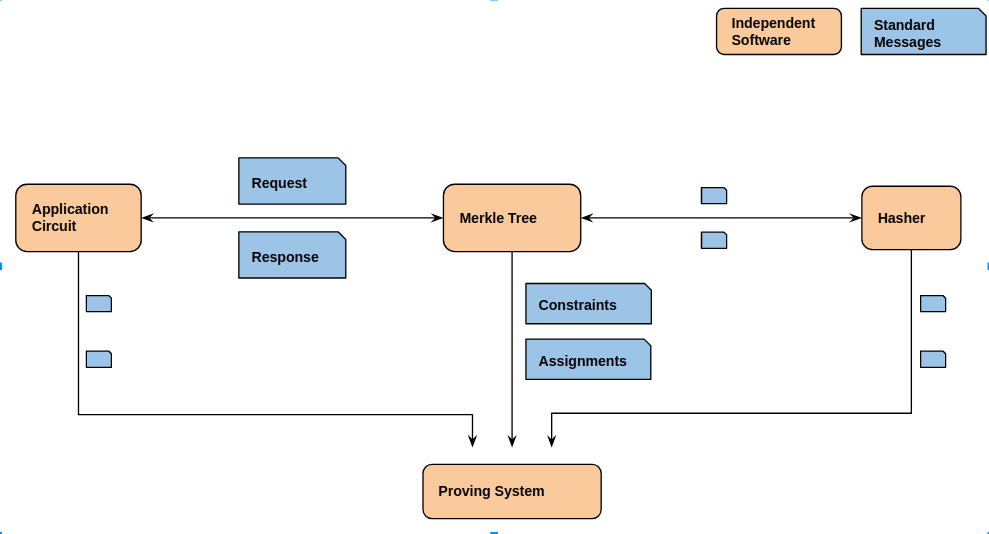
\includegraphics[width=\linewidth]{routine.png}
				\caption{The flow of interaction between existing libraries and the interface}
				\label{flow}
			\end{figure}
		
			here talk about the different levels in word doc

		\paragraph{Instance reduction.} 
		
        Points to include:
        - caller does not provide functionality to gadget and does not depend on specific implementation
        - gadget and caller both allocate variables
		
		\paragraph{Witness reduction.}
		
		r1cs in the format: a way to represent the constraints and a way to represent the assignment; and connection between components (gadgets), which actually are the public inputs. If we think of circuit as components, each component has a set of local inputs and "outgoing" inputs.
		
		So the interface solves two problems: 1/ interop between frameworks (front-ends) and proving systems (backends) 2/ composability of gadgets between different frameworks.
		
	
		
		\subsection{An MVP}
		
		
		
		\subsection{Specification}
		
		*use of flatboard
		
		- semantics; planned parametrization of the semantics.
		
		- format: can work with files (all messages instead of processing, can be written to file) for both instance / witness reduction, otherwise can work with memory 
		
		Each component has an interface; which can be invoked / instantiated / called with other components to make up the constraint system.
			- composibility of gadgets as there local variables / public ones (merkle tree has the leaf and root and invokes sha256)
		
		CRS is specific to proving system so the format does not handle the CRS portability
		
		we are thinking of implementing ZoKrates for the application layer and libsnark, bellman.  
		
		NOTE: some people think of functions, inputs and returned variables; others as circuits and gadgets.
		
		
		Issues: 1/ linear 